\documentclass[conference, a4paper, 10pt, twocolumn]{IEEEtran}
\usepackage{amsmath,amssymb,amsfonts}
\usepackage{algorithmic}
\usepackage{graphicx}
\usepackage{textcomp}
\usepackage{xcolor}
\usepackage[style=ieee]{biblatex}
\usepackage[nottoc]{tocbibind}
\def\BibTeX{{\rm B\kern-.05em{\sc i\kern-.025em b}\kern-.08em
    T\kern-.1667em\lower.7ex\hbox{E}\kern-.125emX}}

\addbibresource{literature_list.bib}
\renewcommand*{\bibfont}{\small}
\begin{document}

\title{Mechanisms to Raise Awareness about Smartwatch Data Collection}

\author{
	\IEEEauthorblockN{
		Mehmed Mustafa
	}
	\IEEEauthorblockA{
		\textit{Institute of Computer Science}\\
		\textit{University of G\"{o}ttingen}\\
		G\"{o}ttingen, Germany\\
		Email: mehmed.mustafa@stud.uni-goettingen.de
	}
	\and
	\IEEEauthorblockN{
		Chris Warin
	}
	\IEEEauthorblockA{
		\textit{Institute of Computer Science}\\
		\textit{University of G\"{o}ttingen}\\
		G\"{o}ttingen, Germany\\
		Email: chris.warin@stud.uni-goettingen.de
	}
}

\maketitle
\thispagestyle{plain}
\pagestyle{plain}


\begin{abstract}
This document is a model and instructions for \LaTeX.
This and the IEEEtran.cls file define the components of your paper [title, text, heads, etc.]. *CRITICAL: Do Not Use Symbols, Special Characters, Footnotes, 
or Math in Paper Title or Abstract.
\end{abstract}

\begin{IEEEkeywords}
component, formatting, style, styling, insert
\end{IEEEkeywords}

\section{Introduction}
Test \cite{shu2016cardea}
\section{Foundations}

The main goal of our work is to raise the awareness about smartwatch data collection. In this section, we first clarify our notion of smartwatch data collection and describe the technologies and platforms we use. A smartwatch is, basically, a device in the form of a watch which has computing capabilities. Although the earlier models had restricted functionality, the models starting from early 2010s are closer to smartphones in regard to features. Modern smartwatches have WiFi/Bluetooth connectivity, support mobile apps, have their own operating system and peripheral devices. Peripheral devices may include health tracking sensors such as heart rate monitors, location tracking sensors such as GPS receivers and activity tracking sensors such as pedometers.\cite{smartwatchWiki}

Mobile apps may gather data from different sensors at any given time. We refer to this process as a smartwatch data collection. Often mobile apps ask for permissions to use different sensors when the app is launched for the first time. Users give permission but are not aware when exactly and how often the app gathers their health, location or activity data. We propose 3 different mechanisms to increase the awareness of the user about the data gathering process: Visual, Sound and Haptic feedback. The visual feedback divides into 3 sub categories: Ring, Icon and Notification. The awareness increasing mechanisms are discussed in more details in secion \ref{Approach}. Our proposal could be further extended and developed as an API which developers 

\begin{figure}[t]
\leftline{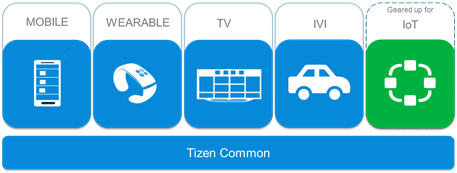
\includegraphics[width=.5\textwidth]{img/tizenInfrastructure.png}}
\caption{Tizen infrastructure}
\label{fig:tizen}
\end{figure}

For our research we use Samsung Galaxy Watch 3 \cite{galaxyWatch3}. The smartwatch runs Tizen OS 5.5\cite{tizenOS}, an open source Linux-based mobile operating system which is built to work on diverse devices. In order to support different types of devices and provide product-optimized performance, Tizen uses different profiles to categorize functions and features according to the requirements of each device type. Currently, four profiles are supported: IoT, Mobile, TV, Wearable. Since all profiles are built on top of a common, shared infrastructure (Fig.~\ref{fig:tizen}), it is easy to add new profiles for emerging technologies. 

Tizen has it's own official IDE for developing web based and native applications. Moreover, the availability of Tizen extensions for Visual Studio Family makes possible to develop Tizen applications in the .NET environment. Tizen .NET, in comparison to web and native frameworks, is more advantageous. The C-based framework does not have advantages of a managed runtime and HTML5-based framework has fewer features supported and worse performance. On the other hand, Tizen .Net has managed runtime advantages such as faster development, safer code, cross-platform support and better quality software. Tizen provides an emulator which increases the application development process. Firstly, because we do not need an actual physical device to start the development process. And secondly, because the control panel of the emulator makes it possible to produce different sensor values.\cite{tizen}



\section{Related Work}

\section{Approach}\label{Approach}

\section{Discussion}

\section{Conclusion}


\begin{figure*}[htbp]
\centerline{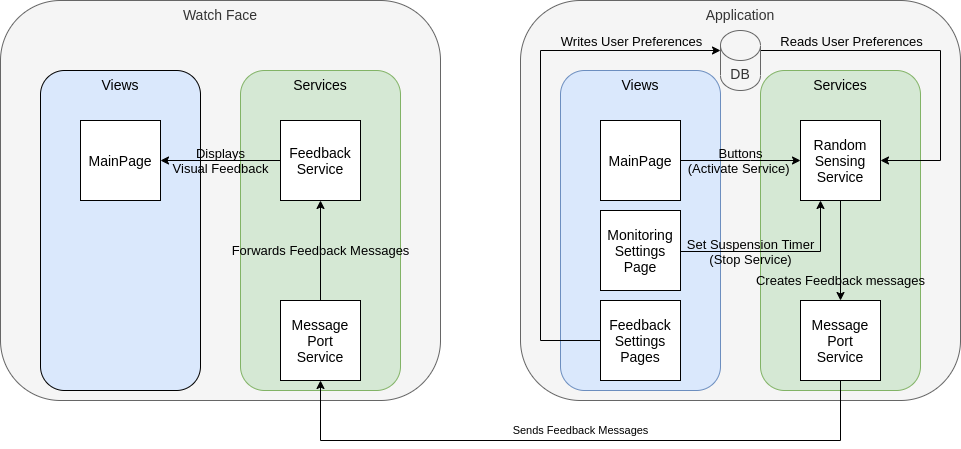
\includegraphics[width=.5\textwidth]{img/appDiagram.png}}
\caption{Example of a figure caption.}
\label{fig}
\end{figure*}

\section*{Acknowledgment}

\printbibliography

\end{document}
